\chapter{Introduction}
\label{sec:introduction}

Beginning in the 1950's, virtual reality technology \cite{steuer1992defining} has been continuously researched and improved and its professional relevance is becoming ever more present today. There is a plenitude of recent works showing that it bears great potential and positive possible contributions to architecture and construction \cite{sampaio2014application}, \cite{le2015social}, \cite{stouffs2013happening}, health care and psychotherapy \cite{baus2014moving}, \cite{merians2014rehabilitation}, \cite{de2014healthcare}, engineering and industrial design \cite{marks2014towards}, \cite{wendrich2016hybrid}, gaming and home entertainment \cite{valente2016live}, \cite{zyda2005visual} and education \cite{merchant2014effectiveness}, \cite{ott2015literature}. One must also consider that this technology can help with gaining new insights and opening up new perspectives into greater, more abstract matters of social, environmental and economic manner \cite{ovtcharova2015innovation}, \cite{nguyen2016applying}. 

With resources such as memory and computing power becoming more and more available at ever-increasing rates, 3D objects and their mesh representations are constantly growing in complexity and size, in terms of shaders, texture maps as well as the sheer number of vertices. Still, many professional applications revolving around interaction with such models require means of displaying them in real-time without significant perceived loss of quality to ensure a smooth and fast workflow. This is where mesh simplification and segmentation plays an important role \cite{wei2010feature}, \cite{shaffer2001efficient}, \cite{zhao2012saliency}.

This issue becomes even more pressing in a professional, commercial context where access to state-of-the-art, high-performance graphic processing units or render farms are not a given for everybody. With less computing power available, means of user-oriented, real-time rendering are of vital importance to a fast and unimpeded way of working on 3D assets. \textit{Mesh saliency} is an automatic, mathematically founded procedure proposed in 2005 by Lee \textit{et al.} \cite{lee2005mesh}. It describes vertex-wise perceived importance a given 3D model, based on differences in local curvature and aims at providing a basis for so-called saliency-based complexity reduction of such objects. Here, the number of vertices and triangles that make up a 3D geometry are automatically reduced, often resulting in gross losses of quality. Concepts such as \textit{mesh saliency} are designed to uphold important details to a certain extent, even after reduction has taking place. Put simply, the idea is to merge more vertices in regions that are deemed to be of low visual interest while keeping the number of vertices high in the important areas.

Lee \textit{et al.} state that their procedure is based on characteristics of human perception and cognition. However, a scientific evaluation as to whether distributions of perceived importance that result from using it are congruent with real impressions of users or not, is yet to be conducted. To tackle this problem, direct user input describing what they perceive as \textit{important}, is needed. This work includes a description of a virtual reality based \textit{selection application} which allows vertex-wise selection of \textit{important} regions.

For this selection process, the Virtual Reality and Visualisation Centre's five-sided projection installation at the Leibniz Supercomputing Centre in Munich was available \cite{v2c}. This installation creates interactive, immersive virtual reality environments via multiple projectors and tracking sensors. Users only need to wear a lightweight pair of stereo shutter glasses that are synchronised with the projectors and thus can seperate two images for the spectator, one for each eye. The glasses are equipped with a tracking system so that their exact position, orientation and tilt can be captured in real-time, allowing computation of the user's perspective into the 3D scene at any time. Based on this perspective, the projectors use the walls as projection surfaces and throw live images resembling what the user would see if he/she were physically in the virtual scene onto the walls. The projection installation grants a virtual reality experience which is enhanced by the fact that the user only needs to wear a pair of glasses instead of a fully sized headset. From a user perspective, another advantage of such a setup is the fact that there are no cables which can evoke a feeling of inhibition or constant worry of stumbling over and accidentally damaging the hardware, connected to the glasses.

This work is segmented into three major tasks. First, a piece of software that allows real-time interaction in an immersive virtual reality environment is implemented. This so-called \textit{selection application} has to let users select and deselect vertices of 3D objects in an easy, fast way and provide clear visual feedback on what is currently selected and what is not. Then, a user study is conducted. Participants are asked to use the \textit{selection application} in the five-sided projection installation of the V2C \cite{v2c} and select parts of three 3D objects that they deem \textit{important}. With this data, a comparison between automatically calculated \textit{importance} (\textit{mesh saliency}) maps and \textit{user saliency} maps can begin. The last step is to start such an evaluation. A measure of difference is conceptualised for this work, trying to describe how much user selections differ from what parts of 3D objects are deemed \textit{interesting} by automatic computation. Based on this measure as well as structured observations of the resulting maps, this evaluation and discussion can begin.

The measure of difference shows that, for the three objects employed during the user study, user selections differ from computed \textit{importance maps} by roughly 23\%, 27\% and 38\%. However, the validity of these ratios can be doubted because the measure of difference, being a first quick suggestion, lacks expressiveness as discussed in section \ref{sec:measure_of_difference}. Furthermore, observations shows that, while there are clear similarities in what is deemed \textit{important} by computation and users, individual, highly object-dependent differences are to be expected.

\begin{figure}[htb]
  \centering
  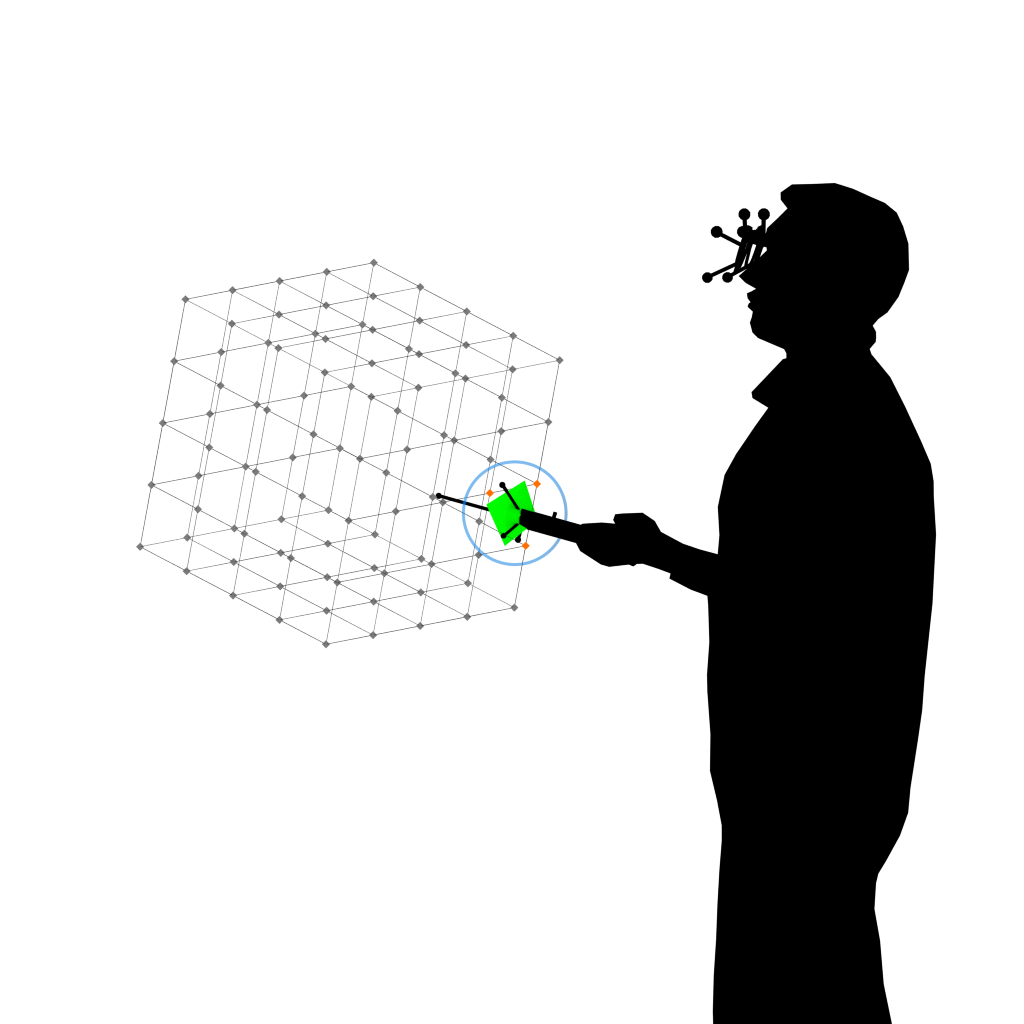
\includegraphics[width=0.8\textwidth]{selection_cave.png}
  \caption{Schematic depiction of how the \textit{selection application} works from a user perspective}
  \label{fig:intro_pic}
\end{figure}

Figure \ref{fig:intro_pic} depicts interaction with the application implemented for this work. Details on its implementation can be found in chapter \ref{sec:selection_application}, the general structure and conceptual part of this work is described in chapter \ref{sec:concept}. For more related work on the topic, see chapter \ref{sec:related_work}.

Details on the user study can be found in chapter \ref{sec:user_study_chapter}, its results are presented and discussed in chapter \ref{sec:results_and_discussion}. Lastly, for a quick summary of this work as well as an outlook on possible future work, see chapter \ref{sec:conclusion_and_future_work}.

